\documentclass[a4paper,10pt]{article}
\usepackage[T1]{fontenc}
\usepackage[utf8]{inputenc}
\usepackage[english]{babel}
\usepackage{lmodern}
\usepackage[top=1.6cm,bottom=1.8cm,left=1.9cm,right=1.9cm]{geometry}
\usepackage{titlesec,enumitem,xcolor,graphicx,lastpage,fancyhdr}
\usepackage{fontawesome5}
\usepackage[hidelinks]{hyperref}
\hypersetup{colorlinks=true,urlcolor=blue!70!black,linkcolor=blue!70!black}
\pagestyle{fancy}\fancyhf{}\renewcommand{\headrulewidth}{0pt}
\fancyfoot[C]{\small\color{gray}Page \thepage\ of \pageref{LastPage}}
\setlength{\parindent}{0pt}
\titleformat{\section}{\large\bfseries}{}{0em}{}[\vspace{-0.7em}\rule{\textwidth}{0.5pt}]
\titlespacing{\section}{0pt}{9pt}{5pt}
\setlist[itemize]{leftmargin=1.1em,itemsep=2pt,topsep=2pt,parsep=0pt}
\newcommand{\role}[4]{\vspace{3pt}\noindent\hspace{0.6em}\parbox[t]{0.38\textwidth}{\raggedright\textbf{#1}}\hfill\parbox[t]{0.58\textwidth}{\raggedleft\textit{#2}}\\{\textit{#3}\hfill\textit{#4}}\vspace{1pt}}
\begin{document}
\noindent
\begin{minipage}[t]{0.78\textwidth}
\vspace{0pt}
{\huge\bfseries Prabhavit Gupta}\\[8pt]
{\small \faPhone\ +39 351 610 7807 \quad \faEnvelope\ \href{mailto:prabhavitg@gmail.com}{prabhavitg@gmail.com} \quad \faLinkedin\ \href{https://www.linkedin.com/in/prabhavit/}{LinkedIn} \quad \faGithub\ \href{https://github.com/prab-gupta}{GitHub} \quad \faMapMarker*\ Venice / Milan, Italy}
\end{minipage}\hfill
\begin{minipage}[t]{0.18\textwidth}
\vspace{0pt}\raggedleft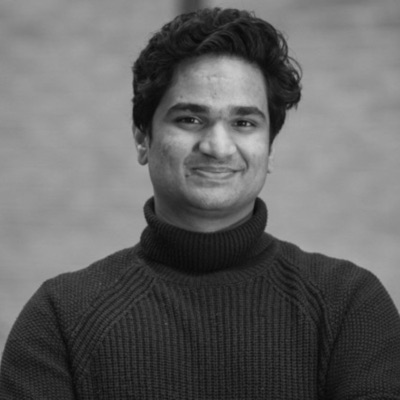
\includegraphics[width=2.3cm]{photo_small.jpg}
\end{minipage}

\section{Career Summary}
\begin{itemize}
\item Forward Deployed Engineer with 3 years of experience deploying real-time communications, voice AI agents, and API integrations for enterprise customers across Southern Europe.
\item Deep technical expertise building low-latency telephony pipelines, WebSockets integrations, Model Context Protocol (MCP) servers, and automated evaluation frameworks.
\item Based in Italy (Venice/Milan), fluent in Italian and English, with full permanent EU work authorization (no visa sponsorship required).
\end{itemize}

\section{Technical Skills}
\begin{itemize}
\item \textbf{Communications AI \& Real-Time Systems} : Voice AI, Real-time Audio/Streaming APIs, WebSockets, WebRTC, SIP Telephony Integrations, Speech-to-Text (STT), Text-to-Speech (TTS), Agentic Tool Calling.
\item \textbf{Software Development} : Python, TypeScript, Node.js, FastAPI, REST APIs, JSON-RPC, Asynchronous I/O.
\item \textbf{Cloud, Infrastructure \& Delivery} : Docker, Linux, CI/CD, Observability \& Telemetry, Automated Testing Harnesses.
\end{itemize}

\section{Professional Experience}

\role{FlowSpace}{Venice / Milan, Italy}{Forward Deployed \& Applied AI Engineer}{11/2024 -- Present}
\begin{itemize}
\item Led customer engineering engagements across Southern Europe, architecting low-latency voice and messaging AI agents for enterprise partners.
\item Designed custom Model Context Protocol (MCP) and WebSocket servers in Python and TypeScript, bridging real-time telephony APIs with LLM reasoning loops.
\item Built automated evaluation suites to continuously audit speech recognition fidelity, latency budgets, and multi-turn conversational tool accuracy.
\item Partnered directly with enterprise engineering leaders to ensure high-availability deployments.
\end{itemize}

\role{UltraStrategy}{Remote, UK/EU}{AI Solutions Engineer}{01/2024 -- 10/2024}
\begin{itemize}
\item Architected and deployed enterprise AI solutions, optimizing token throughput and response latency by 38\%.
\item Authored technical architecture specifications and API documentation for partner integrations.
\end{itemize}

\role{Urlink}{Milan, Italy}{Full Stack \& Automation Engineer}{06/2023 -- 12/2023}
\begin{itemize}
\item Engineered real-time automation microservices and RESTful API integrations handling 100,000+ monthly events.
\item Developed automated testing harnesses that reduced regression rates by 50\%.
\end{itemize}

\role{Get2Germany}{Remote, Germany}{Software Engineer}{08/2022 -- 05/2023}
\begin{itemize}
\item Built full stack applications and backend microservices using FastAPI and PostgreSQL.
\end{itemize}

\section{Education \& Work Authorization}
\begin{itemize}
\item \textbf{Bachelor of Science in Computer Science \& Management} | Universita Ca' Foscari Venezia (2020 -- 2023).
\item \textbf{Work Authorization} : Italian EU Long-Term Residence Permit (\textit{Permesso di Soggiorno UE per Soggiornanti di Lungo Periodo} - permanent resident, unlimited work rights across Italy / EU Remote, zero visa sponsorship needed).
\end{itemize}

\end{document}
